\documentclass[fleqn]{article}
\usepackage{amsmath}
\usepackage[dvips]{graphicx}
\bibliographystyle{plain}
\begin{document}

\section*{\center 1m diameter helium plume}
\subsection*{\underline{Problem Description}}
1m helium plum simulation is a standard test to ensure that CFD algorithm can handle variable density effects, but without extra complications caused by combustion. Validation data for this case is also available~\cite{desjardin}.  At time $t=0$ the computational domain is set up to have 1m diameter helium inlet with air coflow. The rest of the boundaries are set up to simulate open boundaries.
 
\subsection*{\underline{Simulation Specifics}}
\begin{description} 
\item [Component used:] \hfill ARCHES
\item [Input file name:] \hfill helium\_1m.ups
\item [Command used to run input file:]\hfill mpirun -np 64 sus helium\_1m.ups
\item [Postprocessing command:]\hfill scirun helium\_1m.srn

\item [Simulation Domain:]\hfill    3 x 3 x 3 m
\item [Cell Spacing:]\hfill \\ 
2 x 2 x 2 cm (Level 0)

\item [Example Runtimes:] \hfill \\
 8 hours   (64 processors, 2.4 GHz Xeon (inferno cluster))

\item [Physical time simulated:] \hfill 0.97 sec.

\end{description}

\section*{\underline{Results}}
Figure~\ref{results3} shows a 2D center-plane contour plot of density at 
$t=0.97$ seconds. This figure shows what can be expected from the code after
8 hours of run time. Figure~\ref{results4} second helium puff going through
the domain (after 35 hours of run time).
\begin{figure}
\includegraphics[scale=.85]{figures/helium_1m_970.ps}
\caption{2D center-plane contour plot of denisty at $t=0.97$ seconds.}
\label{results3}
\end{figure}
\begin{figure}
\includegraphics[scale=.85]{figures/helium_1m_1750.ps}
\caption{2D center-plane contour plot of density at $t=1.75$ seconds.}
\label{results4}
\end{figure}
\newpage

\bibliography{../references}

\end{document}
